\documentclass[11pt]{article}

\usepackage{amsmath}
\usepackage{amssymb}
\usepackage{amsfonts}
\usepackage{amsthm}
\usepackage{mathtools}
\usepackage{xcolor}
\usepackage{graphicx}
\usepackage[alsoload=binary]{siunitx}
\usepackage{booktabs}
\usepackage{multirow}
\usepackage{fancyvrb}
\usepackage[section]{placeins}
\usepackage{flafter}
\usepackage{microtype}
\usepackage{subfig}
\usepackage{enumitem}
\usepackage{url}
\usepackage{hyperref}

\usepackage{mathpazo}

% a bit more compact
\renewcommand\l{\mathopen{}\left}
\renewcommand\r{\right}

\newcommand\abs[1]{\l\vert #1 \r\vert}

% no section numbers
\setcounter{secnumdepth}{-2}

% leave notes to yourself
\newcommand\todo[1]{\textcolor{red}{\textsc{todo}: #1}}

%%% BLACKBOARD SYMBOLS

\newcommand{\C}{\ensuremath{\mathbb{C}}}
\newcommand{\D}{\ensuremath{\mathbb{D}}}
\newcommand{\F}{\ensuremath{\mathbb{F}}}
\newcommand{\G}{\ensuremath{\mathbb{G}}}
\newcommand{\J}{\ensuremath{\mathbb{J}}}
\newcommand{\N}{\ensuremath{\mathbb{N}}}
\newcommand{\Q}{\ensuremath{\mathbb{Q}}}
\newcommand{\R}{\ensuremath{\mathbb{R}}}
\newcommand{\T}{\ensuremath{\mathbb{T}}}
\newcommand{\Z}{\ensuremath{\mathbb{Z}}}
\newcommand{\QR}{\ensuremath{\mathbb{QR}}}

\newcommand{\Zt}{\ensuremath{\Z_t}}
\newcommand{\Zp}{\ensuremath{\Z_p}}
\newcommand{\Zq}{\ensuremath{\Z_q}}
\newcommand{\ZN}{\ensuremath{\Z_N}}
\newcommand{\Zps}{\ensuremath{\Z_p^*}}
\newcommand{\ZNs}{\ensuremath{\Z_N^*}}
\newcommand{\JN}{\ensuremath{\J_N}}
\newcommand{\QRN}{\ensuremath{\QR_{N}}}
\newcommand{\QRp}{\ensuremath{\QR_{p}}}

%%% GENERAL COMPUTING

\newcommand{\bit}{\ensuremath{\set{0,1}}}
\newcommand{\pmone}{\ensuremath{\set{-1,1}}}

% asymptotics
\DeclareMathOperator{\poly}{poly}
\DeclareMathOperator{\polylog}{polylog}
\DeclareMathOperator{\negl}{negl}
\newcommand{\Otil}{\ensuremath{\tilde{O}}}

\renewcommand{\epsilon}{\varepsilon}

% sets in calligraphic type
\newcommand{\calD}{\ensuremath{\mathcal{D}}}
\newcommand{\calF}{\ensuremath{\mathcal{F}}}
\newcommand{\calH}{\ensuremath{\mathcal{H}}}
\newcommand{\calX}{\ensuremath{\mathcal{X}}}
\newcommand{\calY}{\ensuremath{\mathcal{Y}}}

% types of indistinguishability
\newcommand{\compind}{\ensuremath{\stackrel{c}{\approx}}}
\newcommand{\statind}{\ensuremath{\stackrel{s}{\approx}}}
\newcommand{\perfind}{\ensuremath{\equiv}}

% font for general-purpose algorithms
\newcommand{\algo}[1]{\ensuremath{\mathsf{#1}}}
% font for general-purpose computational problems
\newcommand{\problem}[1]{\ensuremath{\mathsf{#1}}}

%%% "LEFT-RIGHT" PAIRS OF SYMBOLS

% "left-right" pairs of symbols

%% NOTE: this requires \usepackage{mathtools} in the document preamble

% inner product
\DeclarePairedDelimiter\inner{\langle}{\rangle}
% absolute value
% \DeclarePairedDelimiter\abs{\lvert}{\rvert}
% a set
\DeclarePairedDelimiter\set{\{}{\}}
% parens
\DeclarePairedDelimiter\parens{(}{)}
% tuple, alias for parens
\DeclarePairedDelimiter\tuple{(}{)}
% square brackets
\DeclarePairedDelimiter\bracks{[}{]}
% rounding off
\DeclarePairedDelimiter\round{\lfloor}{\rceil}
% floor function
\DeclarePairedDelimiter\floor{\lfloor}{\rfloor}
% ceiling function
\DeclarePairedDelimiter\ceil{\lceil}{\rceil}
% length of some vector, element
\DeclarePairedDelimiter\length{\lVert}{\rVert}
% "lifting" of a residue class
\DeclarePairedDelimiter\lift{\llbracket}{\rrbracket}

%%% CRYPTO-RELATED NOTATION

% KEYS AND RELATED

\newcommand{\key}[1]{\ensuremath{#1}}

\newcommand{\pk}{\key{pk}}
\newcommand{\vk}{\key{vk}}
\newcommand{\sk}{\key{sk}}
\newcommand{\mpk}{\key{mpk}}
\newcommand{\msk}{\key{msk}}
\newcommand{\fk}{\key{fk}}
% \newcommand{\id}{id}
\newcommand{\keyspace}{\ensuremath{\mathcal{K}}}
\newcommand{\msgspace}{\ensuremath{\mathcal{M}}}
\newcommand{\ctspace}{\ensuremath{\mathcal{C}}}
\newcommand{\tagspace}{\ensuremath{\mathcal{T}}}
\newcommand{\idspace}{\ensuremath{\mathcal{ID}}}

\newcommand{\concat}{\ensuremath{\|}}

% GAMES

% advantage
\newcommand{\advan}{\ensuremath{\mathbf{Adv}}}

% different attack models
\newcommand{\attack}[1]{\ensuremath{\text{#1}}}

\newcommand{\atk}{\attack{atk}} % dummy attack
\newcommand{\kr}{\attack{kr}}   % key recovery
\newcommand{\indcpa}{\attack{ind-cpa}}
\newcommand{\indcca}{\attack{ind-cca}}
\newcommand{\anocpa}{\attack{ano-cpa}} % anonymous
\newcommand{\anocca}{\attack{ano-cca}}
\newcommand{\euacma}{\attack{eu-acma}} % forgery: adaptive chosen-message
\newcommand{\euscma}{\attack{eu-scma}} % forgery: static chosen-message
\newcommand{\suacma}{\attack{su-acma}} % strongly unforgeable

% ADVERSARIES
\newcommand{\attacker}[1]{\ensuremath{\mathcal{#1}}}

\newcommand{\Adv}{\attacker{A}}
\newcommand{\AdvA}{\attacker{A}}
\newcommand{\AdvB}{\attacker{B}}
\newcommand{\Dist}{\attacker{D}}
\newcommand{\Sim}{\attacker{S}}
\newcommand{\Ora}{\attacker{O}}
\newcommand{\Inv}{\attacker{I}}
% \newcommand{\For}{\attacker{F}}

% CRYPTO SCHEMES

\newcommand{\scheme}[1]{\ensuremath{\text{#1}}}

% pseudorandom stuff
\newcommand{\prg}{\algo{PRG}}
\newcommand{\prf}{\algo{PRF}}
\newcommand{\prp}{\algo{PRP}}

% symmetric-key cryptosystem
\newcommand{\skc}{\scheme{SKC}}
\newcommand{\skcgen}{\algo{Gen}}
\newcommand{\skcenc}{\algo{Enc}}
\newcommand{\skcdec}{\algo{Dec}}

% public-key cryptosystem
\newcommand{\pkc}{\scheme{PKC}}
\newcommand{\pkcgen}{\algo{Gen}}
\newcommand{\pkcenc}{\algo{Enc}} % can also use \kemenc and \kemdec
\newcommand{\pkcdec}{\algo{Dec}}

% digital signatures
\newcommand{\sig}{\scheme{SIG}}
\newcommand{\siggen}{\algo{Gen}}
\newcommand{\sigsign}{\algo{Sign}}
\newcommand{\sigver}{\algo{Ver}}

% message authentication code
\newcommand{\mac}{\scheme{MAC}}
\newcommand{\macgen}{\algo{Gen}}
\newcommand{\mactag}{\algo{Tag}}
\newcommand{\macver}{\algo{Ver}}

% key-encapsulation mechanism
\newcommand{\kem}{\scheme{KEM}}
\newcommand{\kemgen}{\algo{Gen}}
\newcommand{\kemenc}{\algo{Encaps}}
\newcommand{\kemdec}{\algo{Decaps}}

% identity-based encryption
\newcommand{\ibe}{\scheme{IBE}}
\newcommand{\ibesetup}{\algo{Setup}}
\newcommand{\ibeext}{\algo{Ext}}
\newcommand{\ibeenc}{\algo{Enc}}
\newcommand{\ibedec}{\algo{Dec}}

% trapdoor functions
\newcommand{\tdf}{\scheme{TDF}}
\newcommand{\tdfgen}{\algo{Gen}}
\newcommand{\tdfeval}{\algo{Eval}}
\newcommand{\tdfinv}{\algo{Invert}}
\newcommand{\tdfver}{\algo{Ver}}

%%% PROTOCOLS

\newcommand{\out}{\text{out}}
\newcommand{\view}{\text{view}}

%%% COMMANDS FOR HOMEWORKS

\newcommand{\hwheader}{%
  \chead{\Large \textbf{Homework \hwnum}}

  \lhead{\small
    \textbf{\href{https://t-square.gatech.edu/portal/site/XLS0814164958201208.201208}{Applied
    Cryptography}\\Georgia Tech, Fall 2012}}

  \rhead{\small \textbf{Instructor:
      \href{http://www.cc.gatech.edu/~cpeikert/}{Chris
      Peikert}\\Student: \studentname}}

  \setlength{\headheight}{20pt}
  \setlength{\headsep}{16pt}
  
  \headrule
}


\newcommand\channel{\ensuremath{\mathcal C}}
\newcommand\sschac{\attack{ss-cha-$\channel$}}

% Steganography
\newcommand\stg{\scheme{S}}
\newcommand\stgenc{\algo{SE}}
\newcommand\stgdec{\algo{SD}}



\title{Analysis of Stegosystems}
\author{Sam Britt, Tushar Humbe, Ben Perry, Sanchita Vijayvargiya}
\date{December 7, 2012}

\begin{document}
\maketitle

\section{Introduction}
Steganography effectively hides a message within plain sight, wherein
a message being communicated is hidden inside another ostensibly
innocent message. The message is imperceptible to the adversary that
acts as a regulator within the communication channel. Only the sender
and the receiver situated at either ends of the communication channel
are capable of deciphering existence of the hidden message.

The concept of steganography has been in use since the times of
ancient Greece. Communicating messages concealed underneath the wax of
writing tablets and the technique of dotting successive letters are
some of the ways in which the Greeks steganography. Pirate lore
includes tales of individuals tattooing secret information, such as
maps, on their head which would be covered by their hair. Throughout
World War 2 the grill method was used by the spies. This method
involved wooden templates which would be placed over seemingly
harmless text, revealing the secret message. During the same period,
the Germans devised microdot technology in which a picture could be
printed clearly even after shrinking it to the size of a dot.  At the
time of the British Rule in India, freedom fighters, in order to
communicate with each other used lemon extract to write hidden
messages on a paper containing general information. The hidden message
became visible only when the paper was heated by exposure to a candle
or the sun.

Gustavus Simmons, in 1984, initiated the scientific research on
steganography in ``The Prisoner's Problem and the Subliminal
Channel'' \cite{Simmons1984} where he illustrated the concept of
steganography with the
help of Prisoner's Problem. Two prisoners, Alice and Bob, attempt to
devise a plan to escape even though they are locked up in areas and
are prohibited from engaging in private communication with each other.
Both of the prisoners can correspond merely through a single
communication channel which is scrupulously monitored by the warden of
the prison. The warden, Wendy, is the adversary in this example and is
trying to intercept Alice and Bob's private communications. If Alice
and Bob try to exchange messages that are not completely open to
Wendy, or ones that seem suspicious to her, they will be put into a
high security prison forestalling their plan to escape. Messages sent
without any hidden message are known as covertexts. Messages sent on
the channel containing a hiddentext are known as stegotexts. At this
point, Alice and Bob make use of steganography, by sharing a secret
method or key to hide hiddentexts in some stegotext. Only the two
accomplices are able to decipher the hidden message based on their
secrets, while Wendy remains completely oblivious of that message.

In modern digital steganography, the message is hidden in a digital
file yielding a stegotext. This broad definition is useful because any
message can be embedded in any sort of digital file whether it is
text, photo, or other multimedia. Because this definition does not
define the method in which hiddentext is stored in a stegotext we can
define any method to do the job. However, not all steganographic
methods are steganographically secure. Imagine Alice sending a text
file to Bob and renaming the file extension. At first glance this
could seem like a reasonable message for Alice to send. Upon further
investigation Wendy will be able to identify the hidden message or the
fact that there is a hidden message by comparing this file to other
files of that extension.

In this paper we are going to go over what is needed in a
steganographic model in the first section. After understanding the
model that must be used in stegosystems we will look at the notion of
steganographic security. Next we will look at steganalysis, the act of
analyzing suspected stegotexts to verify the suspicion or obtain the
message. Before concluding, we will look at stegosystems and discuss
issues that these may have in terms of our notions of security.

\section{Steganographic Model}
There are variations in steganographic models, but most papers will
agree that a good model needs to include three parties and a monitored
communication channel. The three active members of the model are
Alice, Bob, and Wendy. Prisoners Alice and Bob are trying to hide a
message, hiddentext, from Wendy the warden. The warden monitors the
communication on the channel and inspects many messages on the
channel. Valid channel messages are known as covertext, these are
messages that should not arouse any suspicion from Wendy. Alice will
run an embedding algorithm on her hiddentext and some covertext to
generate her stegotext. Bob will run an extracting algorithm to obtain
the hiddentext from the stegotext. These are all of the needed pieces
in steganography. If Alice and Bob are able to pass a message which
includes hiddentext through this monitored channel without Wendy
becoming aware of the presence of hiddentext, then Alice and Bob have
successfully sent a stegotext. If Alice and Bob are not trying to hide
a message then they are just sending covertext. Figure~\ref{fig:model}
illustrates steganography in a similar manner to what is described
above.

\begin{figure}[htbp]
  \centering
  \begin{minipage}[t]{.8\linewidth}
    \makebox[\textwidth][c]{
      \input{model.pdf_tex}
    }
    \centering
    \caption{The basic steganographic model. Alice attempts to send
    message $m$ to Bob, concealing it inside the stegotext $C'$.}
    \label{fig:model}
  \end{minipage}
\end{figure}

In order for the steganographic system to function, the following
elements should be present in the model:
\begin{itemize}[noitemsep]
  \item[$C$] Covertext: Has the potential to embed a hiddentext.
  \item[$m$ \& $m'$] Hiddentext: Text to embed in covertext.
  \item[$\stgenc$] Embedding  Algorithm: responsible for producing stegotext.
  \item[$\stgdec$] Extracting Algorithm: responsible for extracting
    hidden text from the stegotext.
  \item[$C'$] Stegotext: Contains hiddentext embedded within.
\end{itemize}

The model above is also known as ``The Prisoner's Problem''. In order
for Alice to send secret messages to Bob, she needs to hide them by
using some covertext in such a way that the warden of the prison,
Wendy, falls short of recognizing anything suspicious about the
message. Wendy is the passive adversary in the stated case. She
performs hypothesis testing to check for anything suspicious by
monitoring both the covertext and stegotext being sent over the
communication channel.

The embedding algorithm $\stgenc$ performs the task of generating
stegotext $C'$ by combining $C$ and $m$. The chief function of the
extracting algorithm $\stgdec$ is obtaining the hidden message $m'$
from $C'$. The extraction of the covertext $C$ is of little importance
at receiver end. In one case,
while Alice is inactive, only the covertext $C$ is sent over the
communication channel to Bob. Embedding does not take place in this
case and the passive adversary Wendy observes a rather innocuous text.
In another case, whilst Alice is active, embedding takes place and the
stegotext that is generated is sent over the communication channel to
Bob. Both Wendy and Bob observe the stegotext $C'$, but only Bob is able
to extract the hidden message from $C'$ with the help of the extracting
algorithm $\stgdec$ that he possesses. In both the cases, Wendy is oblivious
of whether Alice is active or not.

In the above model, an assumption has been made about Alice and Bob
possessing the knowledge of the covertext and the stegotext. Moreover,
the embedding algorithm must always work regardless of the information
that $C'$ holds. Another bold assumption that has been made in this case
is that Bob is somehow aware of when Alice is active, even though he
has no way of doing so. Although it does not affect the outcome, it
does help in understanding the security properties of the
steganographic system.

\section{Steganalysis} 
The goal of steganography is to conceal the fact that two parties are
exchanging confidential information. Unlike cryptography, where the
attackers ``wins'' only if it deciphers and recovers the original
message, an adversary against a steganography systems ``wins'' even if
it realizes the existence of secret message, without having to recover
the hidden text. Steganalysis deals with analyzing the channel to
detect the presence of stego or hidden information. The primary step
is to identify suspected stego media \cite{Das}. The suspected media then
undergoes various transformation and/or modifications in order to
reveal the existence of an embedded message. 

The suspected media is not analyzed by itself without other factors.
An adversary performing the steganalysis will also have knowledge of
all communications within the channel, though an adversary may not
have all that information all the time. There are two classes of
steganography attacks can be used by the snooping adversary Wendy
\cite{Das}.
Wendy may employ a steganography only attack in which he attacker has
access to only the stegotext containing the hidden message. The other
class of attack is the known cover attack in which the attacker has
the original covertext as well as the stegotext. The specific
steganalysis attack will depend on what the hiddentext is contained
in. In the next sections we will look at some common steganographic
applications and methods for analyzing these applications.

\section{Security Definitions}
\subsection{Primitives}
Let $P_X$ be a probability mass function with support $\chi$, where $X$
is a discrete random variable taking the values in $\chi$. The
\emph{entropy} of $X$ is
\begin{equation*}
  H(X) = E\l( -\lg P_X \r),
\end{equation*}
where $E(\cdot)$ is the expected value (weighted average) function;
that is,
\begin{equation}
  H(X) = - \sum_{x\in \chi} P_X(x) \lg P_X(x).
  \label{eq:entropy}
\end{equation}
Intuitively, the entropy of $X$ is a measure of the number of bits of
uncertainty in $X$. For example, suppose $\chi$ is the set of all
$n$-bit strings, and $P_X(x) = 1 / 2^n$ for any $x \in \chi$; that
is, every $n$-bit string is equally likely to be pulled from $P_X$.
This would represent a distribution of maximum uncertainty, and it is
straightforward to show that Eqn.~\eqref{eq:entropy} evaluates to $n$
in this case. In fact, $H(X) = \lg \abs{\chi}$ is an upper bound for
$H$, where $\abs \chi$ denotes the cardinality of $\chi$.

The \emph{minimum entropy} of a distribution $P_X$ is defined as
\begin{equation}
  H_\infty\l( X \r) = \min_{x \in \chi} \l\{ -\lg P_X(x) \r\}
  \label{eq:min-entropy}
\end{equation}
This can be understood as a measure of uncertainty for the ``most
probable'' element in $\chi$ according to $P_X$. For example, if there
is some element $x_0$ with $P_X(x_0) = 1$, then $H_\infty(X) = 0$
(there is no uncertainty in $X$). Suppose the most probable element
$x_0$ has probability $P_X(x_0) = 1/2$. Intuitively, the uncertainty
is unity; that is, we can guess that the next value of $X$ will be
$x_0$ to within a single coin flip. Indeed, evaluating
Eqn.~\eqref{eq:min-entropy} for such a distribution shows that
$H_\infty\l( X \r) = 1$.

Given two probability mass functions $P_X$ and $P_Y$, both with
support $\chi$, the \emph{relative entropy}, also called the
Kullback-Leibler divergence, from $P_X$ to $P_Y$ is defined to be
\begin{equation}
  D \l( P_X \concat P_Y \r) =
  \sum_{x \in \chi} P_X(x) \lg \frac{P_X(x)}{P_Y(x)}.
\end{equation}
Intuitively, the relative entropy is a measure of the difference
between $P_X$ and $P_Y$, although it is important to note that it is
not symmetric; that is, $D \l( P_X \concat P_Y \r) \ne D \l( P_Y
\concat P_X \r)$. However, $D \l( P_X \concat P_Y \r) = 0 $ if and
only if $P_X = P_Y$, and increases indefinitely as $P_Y$ diverges from
$P_X$.

A \emph{channel} as defined by \cite{Hopper2002} is a distribution on
timestamped bit sequences; i.e., a channel \channel\ is a distribution
with support $\set{\l( \bit, t_1 \r), \l( \bit, t_2 \r), \ldots }$,
where each $t_i \le t_{i+1}$. The intent is to model communication,
where not just the content but also the timing of the communication
may be relevant. Since a particular draw from the distribution
\channel\ depends the history of previously drawn bits, define
$\channel_h$ to be the distribution conditioned on history $h$.
Furthermore, it is useful to think of drawing from the channel in
chunks of $b$ bits at a time, so define $\channel_h^b$ to be the
distribution on the next $b$ bits after the history $h$.

\subsection{Security Definitions}
Hopper, et. al \cite{Hopper2002} define a stegosystem $\stg$ as a pair of
randomized algorithms $\l( \stgenc, \stgdec \r)$. $\stgenc$ takes as
input a shared key $k$, a hiddentext message $m$, and a message
history $h$, and an oracle $M(h)$ that samples according to channel
distribution $\channel_h^b$, where channels are required to satisfy,
for all $h$ drawn from \channel, $H_\infty\l( \channel_h^b \r) > 1$.
As output, $\stgenc_k^M\l( m, h \r)$ returns a sequence $c_1 \concat
c_2 \concat \ldots \concat c_\ell$ in the support of $\channel_h^{\ell
b}$. The decryption algorithm $\stgdec_k^M\l( c_1 \concat c_2 \concat
\ldots \concat c_\ell, h \r)$ returns a message $m$, which should be
``correct''; that is, the same message encoded by $\stgenc$, at least
$2/3$ of the time.

The authors define the security of a stegosystem in terms of a game.
The adversarial warden $W$ is given access to $M\l( h \r)$, which
returns draws from $\channel_h^b$, and an oracle $\Ora$. The oracle
$\Ora$ is either $\stgenc_k$ or a function $O(\cdot, \cdot)$, where
$O(m, h)$ simply returns a draw from $\channel_h^{\abs{\stgenc_k\l( m,
h \r)}}$. The warden also has access to randomness $r$. The warden's
advantage against the steganographic secrecy under chosen hiddentext
attack for channel $\channel$ of stegosystem $\stg$ is defined by
Hopper et.\ al to be
\begin{align*}
  \advan_{\stg, \channel}^\sschac \l( W \r) = \abs {
  \Pr_{k, r, M, \stgenc} \l[ W_r ^{M, \stgenc_k(\cdot, \cdot)}
  \text{accepts} \r]
  -
  \Pr_{r, M, O} \l[ W_r ^{M, O(\cdot, \cdot)}
  \text{accepts} \r]
}.
\end{align*}
A stegosystem $\stg$ is \emph{$(t, q, \ell,
\epsilon)$-steganographically secret under chosen hiddenttext attack}
for channel $\channel$ (SS-CHA-$\channel$) if, for any warden $W$
making at most $q$ queries totaling at most $\ell$ bits of hiddentext,
and running in time at most $t$,
\begin{equation*}
  \advan_{\stg, \channel}^\sschac\l( W \r) \le \epsilon;
\end{equation*}
that is, the stegosystem $\stg$ is insecure if an efficient warden can
(with high probability) distinguish between the output of
$\stgenc_k(m, h)$ and draws from $\channel_h^{\abs{\stgenc_k(m,h)}}$,
even when given access to $\channel_h^b$ through $M$. A stegosystem
$\stg$ is \emph{$(t, q, \ell, \epsilon)$-universally
steganographically secret under chosen hiddenttext attack} for channel
$\channel$ (USS-CHA-$\channel$) if it is $\l( t, q, \ell,
\epsilon\r)$-SS-CHA-\channel\ for any channel \channel\ that
satisfies, $\forall h$ drawn from \channel, $H_\infty\l( \channel_h^b
\r) > 1$.

Cachin \cite{Cachin2004} takes an information theoretic approach to
steganographic security. He considers the basic prisoner's problem,
where Alice sends either an innocent covertext or a stegotext
concealing a message to Bob over an open communication line. The
warden eavesdrops on the line, and must decide whether the
communication is a covertext or stegotext. Let $P_C$ be the
distribution of covertexts, and let $P_S$ be the distribution of
stegotexts; these distributions are known to the warden. Cachin
defines the overall security of the system in terms of the relative
entropy between $P_C$ and $P_S$; namely, the stegosystem is
\emph{information-theoretic perfectly secure} if
\begin{equation*}
  D\l( P_C \concat P_S \r) = 0,
\end{equation*}
and is \emph{information-theoretic $\epsilon$-secure} if
\begin{equation*}
  D\l( P_C \concat P_S \r) \le \epsilon.
\end{equation*}
Intuitively, Cachin is claiming that a stegosystem is secure if the
probability distributions of covertexts and stegotexts are ``close,"
so that, given a message in the support of $P_C$ and $P_S$, the
warden has very little reason to believe it was drawn from one
distribution over the other. Cachin goes on to analyze the decision
from the framework of hypothesis testing.

Cachin's warden is a much weaker adversary than Hopper's, and
correspondingly, Hopper's SS-CHA-\channel\ game provides a much
stronger definition of security. Some key weaknesses in Cachin's
definition:
\begin{itemize}
  \item Cachin's warden receives a single message over the
    communication line, and must determine her decision. In contrast,
    Hopper's warden has access to an oracle that can be queried as
    much as is computationally feasible. Indeed, Cachin's model is
    roughly equivalent to the SS-CHA-\channel\ game when only a single
    query is allowed.
  \item Cachin's warden knows the distribution of possible messages
    chosen by Alice, but does not know the message. Hopper, however,
    allows for an interactive, chosen hiddentext attack.
  \item Hopper's channels are all conditioned on the \emph{history} of
    previously drawn samples. And since his warden is allowed to
    specify arbitrary history to the oracles, a stegosystem that meets
    SS-CHA-\channel\ security should be secure for any valid history
    of communication on \channel. On the other hand, Cachin's model,
    because it depends on static probability distributions, does not
    capture this sequential element of real communication. Even if
    $P_C$ and $P_S$ were themselves dependent on history, Cachin's
    model would only be able to claim security of the stegosystem for
    the particular history leading up to his experiment.
\end{itemize}

Though Cachin's definitions are weaker, they are not without merit.
Hopper's security schemes require perfect oracles---oracles that can
sample from $\channel_h$ for arbitrary $h$, can be ``rewound," etc.
Given the application, the lack of such an available oracle may make
implementation of security schemes (and proof of their security)
difficult or impossible. In contrast, knowledge about $P_S$ and
$P_C$ might be easier to determine for a scheme couched in Cachin's
framework.

\section{Steganographic Applications}
Over the years, various steganography techniques have been used to
send secret messages, embedded in innocuous media. The applications
exploit the structure of the media to conceal sensitive information.
Common modern techniques of steganography can be classified as image
steganography, audio and video steganography, text steganography and
network steganography.

\subsection{Image Steganography}
Hiding information in digital images is one of the most popular
steganography techniques. A digital image is a representation of
pixels. Pixels are typically made of three color channels, for example
red-green-blue, and each color channel will have have an intensity
assigned to it. One color channel is normally 8 bits wide, but the
size can vary. Changing the least significant bit (LSB) of each color
channel intensity will change the resulting pixel very slightly.
Steganographic applications can encode three bits of binary data into
every pixel in an image. The change will likely not be detectable by
the human eye. There are various variations in this techniques. The
number of bits per pixel can be varied or several pixels could be used
to hide one bit of information. Sometimes a fixed number of pixels,
previously decided by the two parties, are skipped to provide more
obscurity.

Still image steganography is susceptible to various known-cover
attacks. Analyzing the cover image and the stego image can reveal the
existence of hidden message. For example, the GIF image format uses
only 8-bits per pixel and changing the LSB can result in large change
in the intensity of the pixel \cite{Meghanathan}. Cmorik and Sum\'ak
\cite{Cmorik} demonstrate various structural and visual techniques to
reveal modification of the original image. For example, changing the
image pixels to a black and white scale reveals modifications in the
LSB, and thus the stegotext \cite{Cmorik} (see Figure~\ref{fig:stego-image}).

\begin{figure}[htbp]
  \centering
  \begin{minipage}[t]{.7\linewidth}
    \centering
    \subfloat[The image on the left is the original image, while the
    one on the right is the stego image.]{
      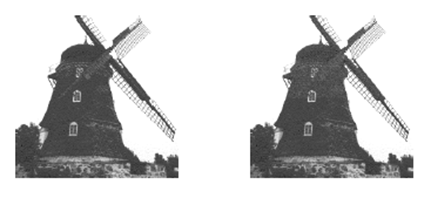
\includegraphics[width=\linewidth]{greyscale}
    }\\
    \subfloat[Changing the pixels to a black and white scale reveals
      the fact that the image on the right contains secret message in
      the first half of the pixels.]{
      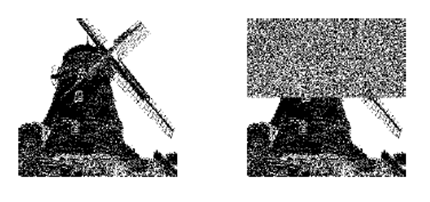
\includegraphics[width=\linewidth]{bw}
    }
    \caption{An example of steganalysis via conversion from greyscale
    to black-and-white.}
    \label{fig:stego-image}
  \end{minipage}
\end{figure}

If the location of the bit(s) in an image does not change then simple
attacks can run against the stegosystem and win with ease. The
simplest attack would be to look in those locations when calling the
oracle with  the all 1's message and the all 0's message. If the
location of the bit(s) is unchanging we can expect that the two
locations will be different even if the coverimage is new.

\subsection{Text Steganography}
\label{sub:text_steganography}
Text steganography involves hiding messages in plain text or text
documents using certain predefined schemes like selected characters,
special symbols, extra white spaces, position of tag attributes in
html documents etc. 

Dulera, et. al \cite{Dulera} explain several techniques used in text
steganography. For example, the alphabet space is divided into two
parts, say letters with a curvature in a shape (B, C, Q), that
represent bit ``0'', while others (A, M, T), represent bit ``1''. Alice
and Bob will then exchange messages by embedding a bit in the first
letter of the sentences. Thus if Alice wants to send ``101'' to Bob, the
transmitted stegotext might look something like

\begin{quote}
  \itshape Today is a holiday. Burger at Wendy's. My Treat!
\end{quote}

Such a stegosystem fails Hopper et.\ al's definition of security
immediately. A warden could launch a simple attack: query the oracle
on a hiddentext of all ones, and arbitrary history. If the oracle
returns a text where every sentence begins with letter without
curvature, accept, otherwise, reject. In the case that the oracle is
the steganographic embedding algorithm, the warden will always accept.
In the case that the oracle is not, then the probability of accepting
is the probability that a draw from the channel returns such a
sentence, which is unlikely for normal English communication.

Such a scheme is exemplary of the kinds of heuristic schemes that rely
so heavily on obscurity and not actual security. The success of such a
scheme in practice relies completely on a warden that is perhaps not
overly suspicious, or is unaware of the algorithms used in the
encryption scheme.

Messages have also been embedded in HTML documents using the html tag
attributes. This approaches exploits the structure of an HTML document
as well as the properties of the media, that is the Internet, to hide
and share information. Garg \cite{Garg2011} demonstrates various approaches
of concealing information in HTML documents. For example, if an html
tag has the ``class'' attribute before the ``style,'' it represents
bit ``0,'' else bit ``1.'' Thus it exploits the fact that changing the
order of the attribute does not change the appearance of the document.
Also the popularity of the internet and the high percentage of tags in
an HTML document, allows you to communicate secret messages with ease.
However, the scheme fails under chosen hiddentext attack in the same
manner as above.

\subsection{Audio and Video Steganography}
Improvement in the Voice over Internet Protocol (VoIP) and other
peer-to-peer~(P2P) protocols make hiding information in audio signals
possible. Furthermore, audio signals contain a large amount of
unpredictable random noise, facilitating covert communication
\cite{Meghanathan}. A
video signal consists of audio and images. Thus, most of the
techniques used in Image and Audio Steganography can be applied to
modify a video signal. Some of the common techniques in audio and
video steganography are briefly described below.

As with image steganography the least significant bit can be used to
encode secret messages. Similar to images, each bit of the hiddentext
is embedded in the LSB of each sample. This minor change cannot be
distinguished by the human visual or auditory system. Given the same
oracle access as before Wendy should be able to differentiate the real
world and the random world without much difficulty if she knows where
to look for the hiddentext, in the LSB.
 
Phase encoding makes small changes in the audio signal phase which are
difficult for the human auditory system to detect, making it a good
place to hide a message. The secret message bits are encoded as phase
shifts in the digital signal\cite{Das}. If the phase shifts only exist in
stegotext, then winning the game are trivial for Wendy. However if
arbitrary phase shifts occur commonly in covertext, then this task
becomes much harder. Periodicity of phase changes could help to
identify the stegotext by varying the length of the hiddentext and
looking for phase changes.

The last common method that we will look at is echo hiding. An echo
consists of three parts that can be manipulated to hide information.
The three parameters of an echo are amplitude, decay rate, and delay.
Echoes must have minimum delay to be heard by the human ear. If a
delay smaller than this is used then these echoes are not perceived by
the human ear. Because this technique adds faint, possibly
imperceptible, echoing to the original covertext, this method requires
higher data transmission rate and quality for the transmitted
stegotext\cite{Meghanathan}. The binary message to be hidden is
embedded in the delay parameter of the echo.

Audio and video steganalysis techniques are limited due to the
advancement in audio steganography and the nature of audio/video
signals which can consists a high percentage of noise and other
unpredictable random bits. In \emph{Steganalysis Algorithms for
  Detecting the Hidden Information in Image, Audio and
Video}\cite{Meghanathan}, Meghanathan and Nayak list various audio and
video steganalysis techniques related to frequency analysis, signal
distance measurement, phase and audio analysis. They also state
various frame correlation analysis algorithm and other video
steganalysis techniques.

\subsection{Network Steganography}
A TCP/IP datagram header contains various fields, which can be used
for hiding data. \emph{Steganography and Steganalysis: Different
Approaches} \cite{Szczypiorski} demonstrates how various IP datagram fields
like Flag, Identification and Initial Sequence Number (ISN) can be
used to hide information in the network packet. Similarly the packet
structure of the Internet Control Message Protocol (ICMP) can be
exploited to send secret information.

However, various packet analysis techniques have been developed to
detect network steganography. Unusual patterns are developed in case
of using TCP/IP packets for network steganography and the presence of
hidden information can be detected \cite{Das}. As seen before, stegosystems
that use non-random placement of bits can be easily detected by Wendy.
Algorithms like this have better security if, instead of hiding the
message bit-by-bit in known locations, an entire IP payload is random
output that hashes to a single bit. The Warden will still be
suspicious of the garbled output, but depending on the channel it
could be expected.

\section{Conclusion}
Stegosystems have existed for a long time. The idea of hiding a
message in plain sight is useful when just the act of hiding a message
is problem enough. The prisoner game with Alice, Bob, and Wendy is the
common model for boiling down steganographic systems to their base
components. From this model we are able to understand the notions of
security tied to steganographic systems. Although each implementation
of steganography can be different, steganalysis is the act of looking
for the existence of hiddentext as well as the actual hiddentext. Some
of the common covertexts include multimedia and text itself. We went
over some applications that use these as covertexts and look at why
they seem to be invalid for security.

We see that perfect stegosystems are difficult to implement because
Wendy can win by identifying a communication as being a stegotext.
This makes the channel and stegosystem very important. Arbitrary
implementations like we have seen above are famous for demonstrating
basic steganography, but offer little in the way of a secure
stegosystem.

\bibliographystyle{elsarticle-num}
\bibliography{Stego}

\end{document}
